%%%%%%%%%%%%%%%%%%%%%%%%%%%%%%%%%%%%%%%%%
% baposter Portrait Poster
% LaTeX Template
% Version 1.0 (15/5/13)
%
% Created by:
% Brian Amberg (baposter@brian-amberg.de)
%
% This template has been downloaded from:
% http://www.LaTeXTemplates.com
%
% License:
% CC BY-NC-SA 3.0 (http://creativecommons.org/licenses/by-nc-sa/3.0/)
%
%%%%%%%%%%%%%%%%%%%%%%%%%%%%%%%%%%%%%%%%%

%----------------------------------------------------------------------------------------
%	PACKAGES AND OTHER DOCUMENT CONFIGURATIONS
%----------------------------------------------------------------------------------------

\documentclass[a0paper,portrait]{baposter}

\usepackage[font=footnotesize,labelfont=bf]{caption} % Required for specifying captions to tables and figures
\usepackage{booktabs} % Horizontal rules in tables
\usepackage{relsize} % Used for making text smaller in some places
\usepackage[utf8x]{inputenc}
\usepackage[superscript,biblabel]{cite}
\usepackage{amsmath}


\graphicspath{{figures/}} % Directory in which figures are stored

\definecolor{bordercol}{RGB}{40,40,40} % Border color of content boxes
\definecolor{headercol1}{RGB}{186,215,230} % Background color for the header in the content boxes (left side)
\definecolor{headercol2}{RGB}{80,80,80} % Background color for the header in the content boxes (right side)
\definecolor{headerfontcol}{RGB}{0,0,0} % Text color for the header text in the content boxes
\definecolor{boxcolor}{RGB}{186,215,230} % Background color for the content in the content boxes

\begin{document}

\background{ % Set the background to an image (background.pdf)
\begin{tikzpicture}[remember picture,overlay]
\draw (current page.north west)+(-2em,2em) node[anchor=north west]
{
\includegraphics[height=1.1\textheight]{background.pdf}};
\end{tikzpicture}
}

\begin{poster}{
grid=false,
borderColor=bordercol, % Border color of content boxes
headerColorOne=headercol1, % Background color for the header in the content boxes (left side)
headerColorTwo=headercol2, % Background color for the header in the content boxes (right side)
headerFontColor=headerfontcol, % Text color for the header text in the content boxes
boxColorOne=boxcolor, % Background color for the content in the content boxes
headershape=roundedright, % Specify the rounded corner in the content box headers
headerfont=\Large\sf\bf, % Font modifiers for the text in the content box headers
textborder=rectangle,
background=user,
headerborder=open, % Change to closed for a line under the content box headers
boxshade=plain
}
{}
%
%----------------------------------------------------------------------------------------
%	TITLE AND AUTHOR NAME
%----------------------------------------------------------------------------------------
%
{\sf\bf \huge{A comparative analysis of Chikungunya and Zika transmission}} % Poster title
{ \underline{Julien Riou}, Chiara Poletto, Pierre-Yves Boëlle\\ % Author names
{\smaller \textit{ Sorbonne Universités, Inserm/UPMC, Institut Pierre Louis d’Epidémiologie et de Santé Publique (IPLESP UMRS 1136), Paris, France} \\ 
 \small{[ julien.riou@iplesp.upmc.fr ]}}} % Author email addresses
{
\includegraphics[scale=.25]{logos2.pdf}} % University/lab logo

%----------------------------------------------------------------------------------------
%	INTRODUCTION
%----------------------------------------------------------------------------------------

\headerbox{Introduction}{name=introduction,column=0,row=0}{
\begin{flushleft}

The recent global dissemination of Chikungunya and Zika has fostered public health concern worldwide. 
To better understand the drivers of transmission of these two arboviral diseases, we propose 
a joint analysis of Chikungunya and Zika epidemics in the same territories, taking into account the common 
epidemiological features of the epidemics: transmitted by the same vector, in the same environments, and observed by the same surveillance systems. 

\begin{center}
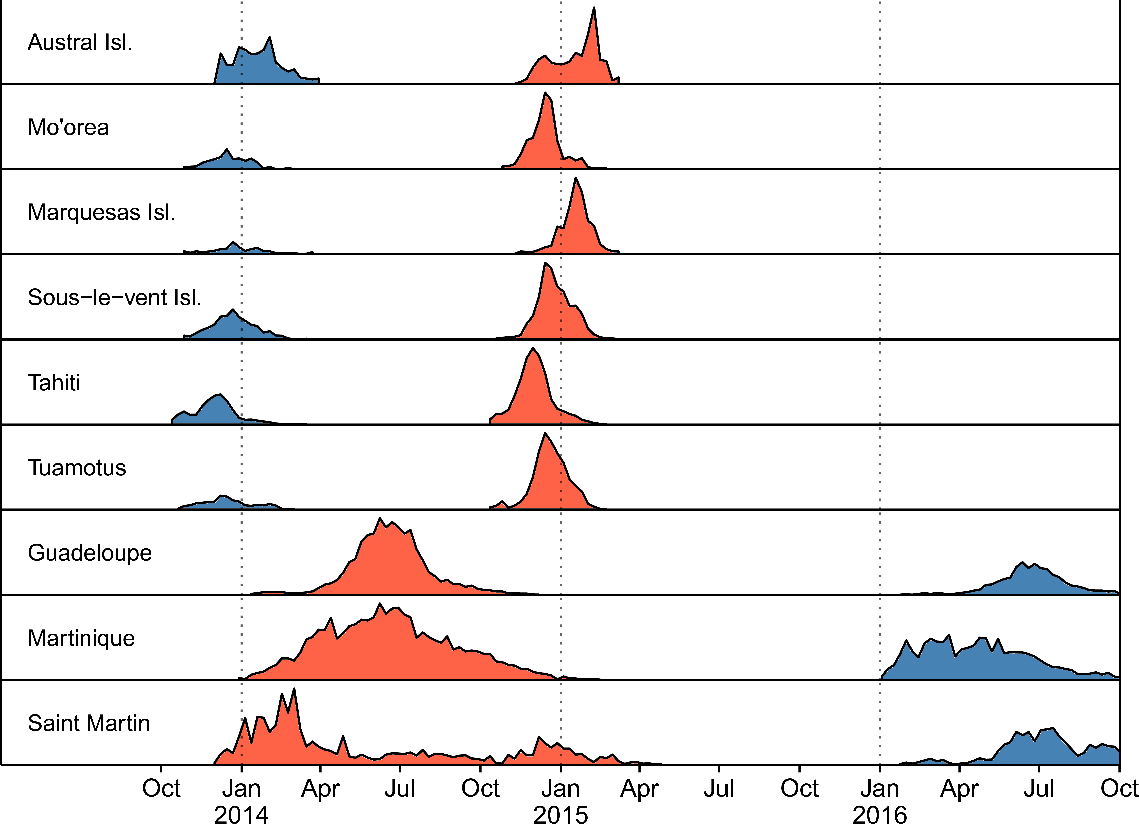
\includegraphics[width=.95\linewidth]{figures/Fig1_revised22.pdf}
\captionof{figure}{{ Profiles of CHIKV (red) and ZIKV (blue) outbreaks in the nine territories under study.}}
\end{center}


\end{flushleft}
}

%----------------------------------------------------------------------------------------
%	MATERIALS AND METHODS
%----------------------------------------------------------------------------------------

\headerbox{Materials and Methods}{name=methods,column=0,below=introduction}{
\begin{flushleft}

We analysed the Zika and Chikungunya epidemics occurring between 2013 and 2016 in 6 islands of French Polynesia and 3 islands of the French West Indies by fitting weekly incidence data with a common hierarchical transmission model.
The two main components of this analysis were: \\
(1) a mechanistic reconstruction of the \textbf{distribution of the serial interval} of the diseases including the influence of temperature; \\
%
%\begin{center}
%\includegraphics[width=.95\linewidth]{figures/Fig22.pdf}
%\captionof{figure}{{Mean, 2.5\% and 97.5\% quantiles of the serial interval duration for CHIKV (A) and ZIKV (B) according to temperature (in $^{\circ}$C).}}
%\end{center}

(2) \textbf{a hierarchical TSIR model} \cite{perkins_estimating_2015} for the generation of observed secondary cases $O_{ijt}$ accounting for the respective effect of virus $j$, location $j$ and weather conditions at time $t$:
\begin{equation*}
O_{ijt} \sim \mbox{NegBin} \left(R_{0ijt} \frac{S_{ijt}}{N_j}\sum_{n=1}^5 w_{it,n} O_{ij,t-n}, \phi \right)
\end{equation*}
where:  the transmission parameter $R_{0ijt}$ depends on an island-specific random intercept, on the relative effect of ZIKV on transmission (compared to CHIKV), and possibly on weather conditions;
$S_{ijt} / N_j$ is the proportion of susceptible at time $t$ (which depends on cumulative incidence until date $t-1$ and on $\rho_{ij}$, the reporting rate parameter, also with an island-specific random component);
and $\sum_{n=1}^5 w_{t,n} O_{t-n}$ summarizes exposure to infectious mosquitoes at time $t$ (i.e. observed incidence in the last five weeks weighted by the discretized distribution of the serial interval).
The model was implemented in \textit{Stan}\cite{carpenter2015stan} using weakly-informative priors.
%\item and $\sum_{n=1}^5 w_{t,n} O_{t-n}$ summarizes exposure to infectious mosquitoes at time $t$ (i.e. observed incidence in the last five weeks weighted by the distribution of the serial interval).
% the transmission coefficient $\beta_{ijt}$ depends on an island-specific random parameter for CHIKV, a parameter for the relativeZIKV, and 
%\item the probability that a case is reported to the surveillance system (random effect);
%\item the number of observed cases in the five preceding weeks, weighted by the distribution of the serial interval;
%\item the proportion of susceptibles;
%\item a transmission coefficient that included the respective influence of the island (random effect), of the virus and of local meteorological conditions on transmission.


\end{flushleft}
}

%----------------------------------------------------------------------------------------
%	CONCLUSION
%----------------------------------------------------------------------------------------

%\headerbox{Conclusion}{name=conclusion,column=0,below=methods}{
%
%}

%----------------------------------------------------------------------------------------
%	REFERENCES
%----------------------------------------------------------------------------------------
%
\headerbox{References}{name=references,column=0,below=methods}{

\smaller % Reduce the font size in this block
\renewcommand{\section}[2]{\vskip 0.05em} % Get rid of the default "References" section title
\nocite{*} % Insert publications even if they are not cited in the poster

\bibliographystyle{unsrt}
\bibliography{sample} % Use sample.bib as the bibliography file
}

%----------------------------------------------------------------------------------------
%	ACKNOWLEDGEMENTS
%----------------------------------------------------------------------------------------

%\headerbox{Contact}{name=acknowledgements,column=0,below=references, above=bottom}{
%
%\smaller % Reduce the font size in this block
%Julien Riou, M.D., PhD candidate \\
%julien.riou@iplesp.upmc.fr
%+336 67 50 94 59
%} 

%----------------------------------------------------------------------------------------
%	RESULTS 1
%----------------------------------------------------------------------------------------

\headerbox{Results: model fit and parameter estimates}{name=results1,span=2,column=1,row=0}{ % To reduce this block to 1 column width, remove 'span=2'

The {\em baseline} model (without the influence of weather) captured the essential characteristics of the outbreaks, as shown in Fig. 2. 

\begin{center}
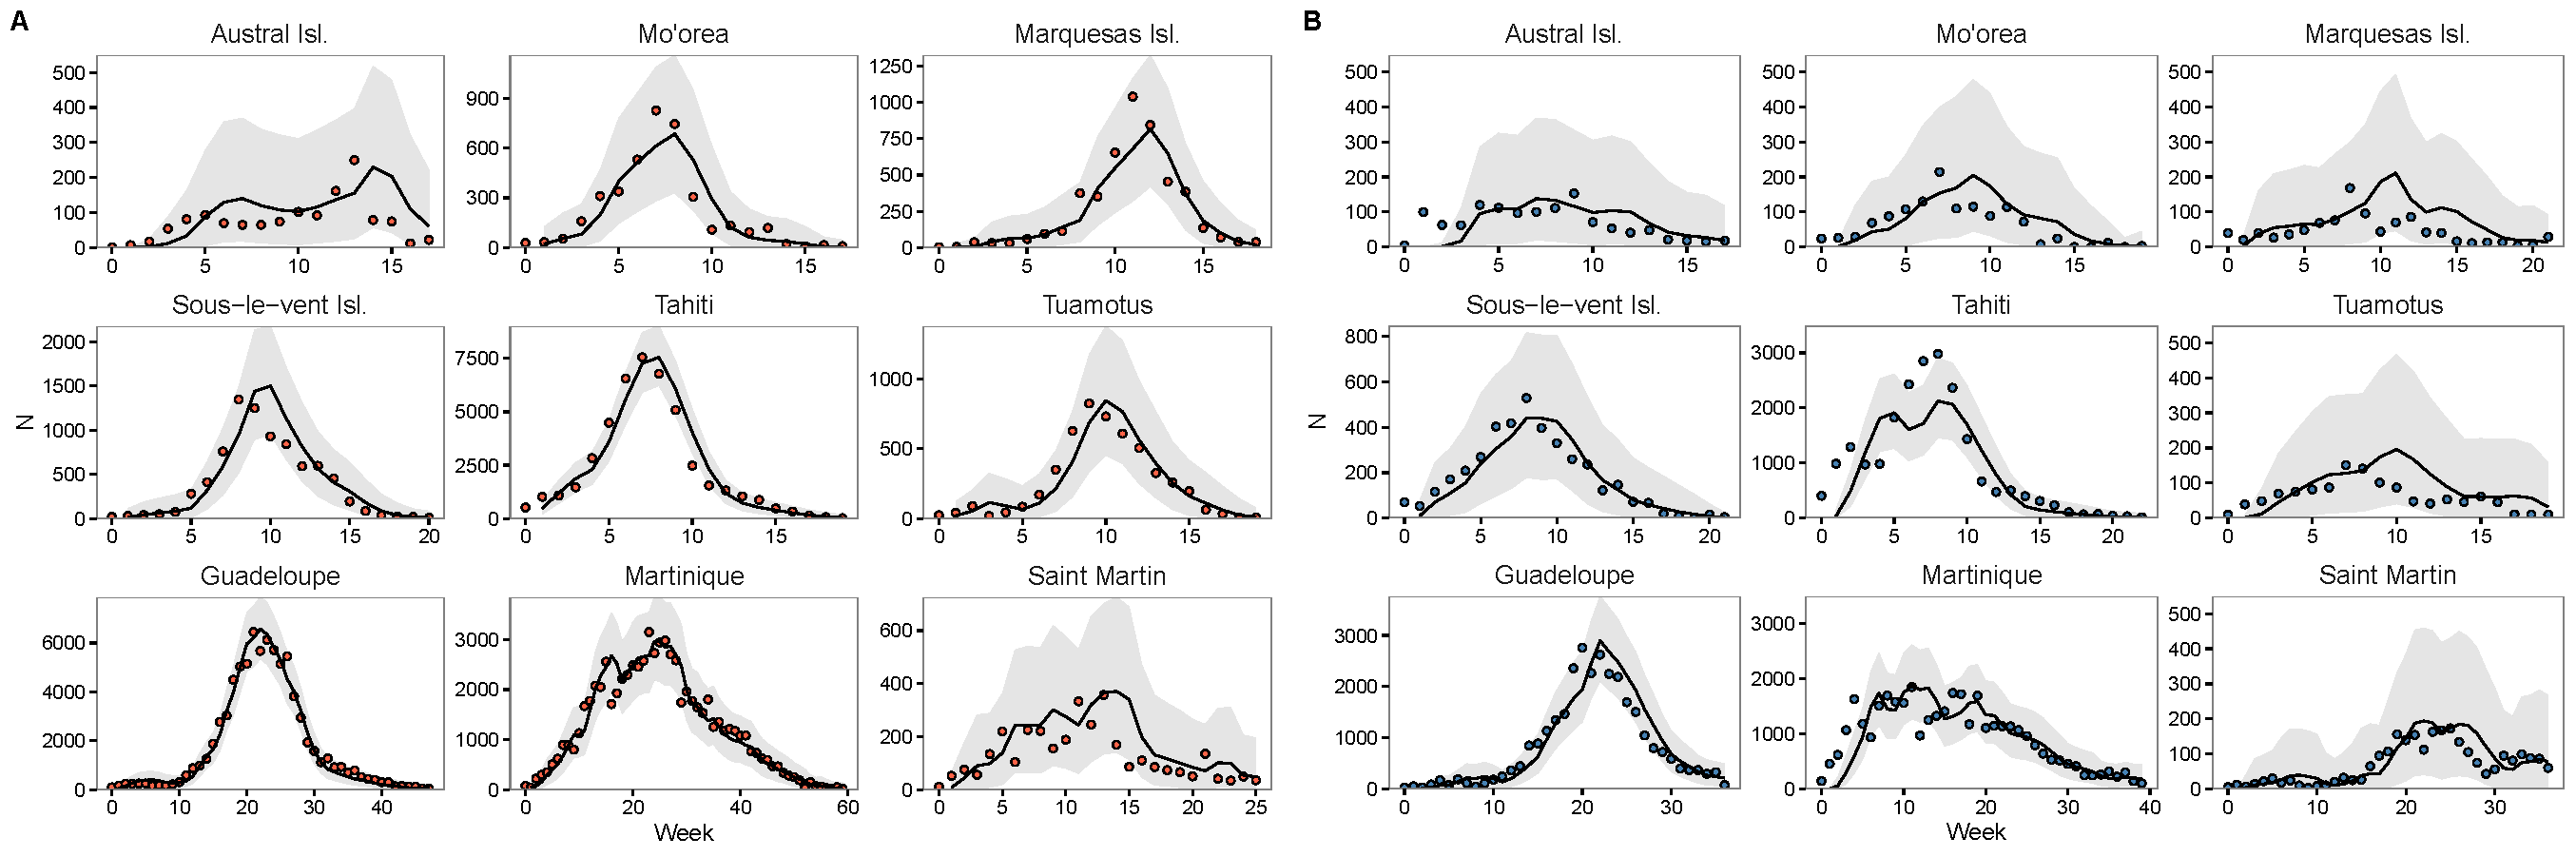
\includegraphics[width=.95\linewidth]{figures/Fig3_poster.pdf}
\captionof{figure}{{Observed numbers of clinical cases (circles) for CHIKV (panel A) and ZIKV (panel B), and corresponding predicted values from the baseline model.}}
\end{center}

The island-averaged reporting rate $\bar{\rho}$ differed according to the disease, estimated at 40\% [29\%; 54\%] for CHIKV and 19\% [12\%; 28\%] for ZIKV. 
The transmissibility ratio between ZIKV and CHIKV was 1.04 [95\%CI: 0.97; 1.13], showing no significant difference in transmissibility between the diseases. Indeed, the island-averaged reproductive ratio was $\bar{R}_0=$ 1.80 [1.54; 2.12] for CHIKV and 1.88 [1.59; 2.22] for ZIKV. 
The variance for the random island effects in reporting and in transmission were different from 0, indicating heterogeneity between locations (Fig. 3).

\begin{center}
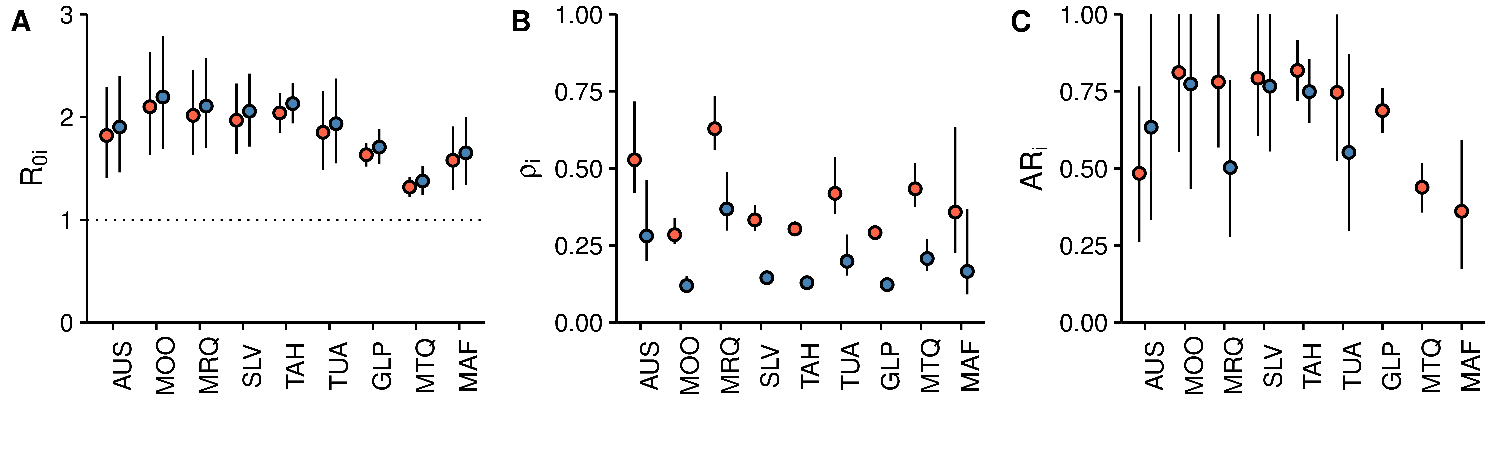
\includegraphics[width=.85\linewidth]{figures/Fig4_revised2.pdf}
\captionof{figure}{{(A) Island-specific basic reproduction ratio $R_{0i}$; (B) reporting rate $\rho_i$; and (C) final attack rate $AR_i$ for CHIKV (red) and ZIKV (blue).}}
\end{center}


}

%----------------------------------------------------------------------------------------
%	RESULTS 2
%----------------------------------------------------------------------------------------

\headerbox{Results: weather conditions and disease transmission}{name=results2,span=2,column=1,below=results1}{ % To reduce this block to 1 column width, remove 'span=2'

We added all combinations of precipitation and temperature on transmission with a lag of up to 8 weeks, and compared models using LOOIC values. Including precipitation in transmission improved the fit (LOOIC difference = -18, standard error = 17), while the effect of temperature was not meaningful (LOOIC difference = +2, se = 13).
The effect of local precipitation showed a marked pattern on transmission, with higher rainfall decreasing transmission one to two weeks later and then increasing transmission four to six weeks afterwards (Fig. 4).

\begin{center}
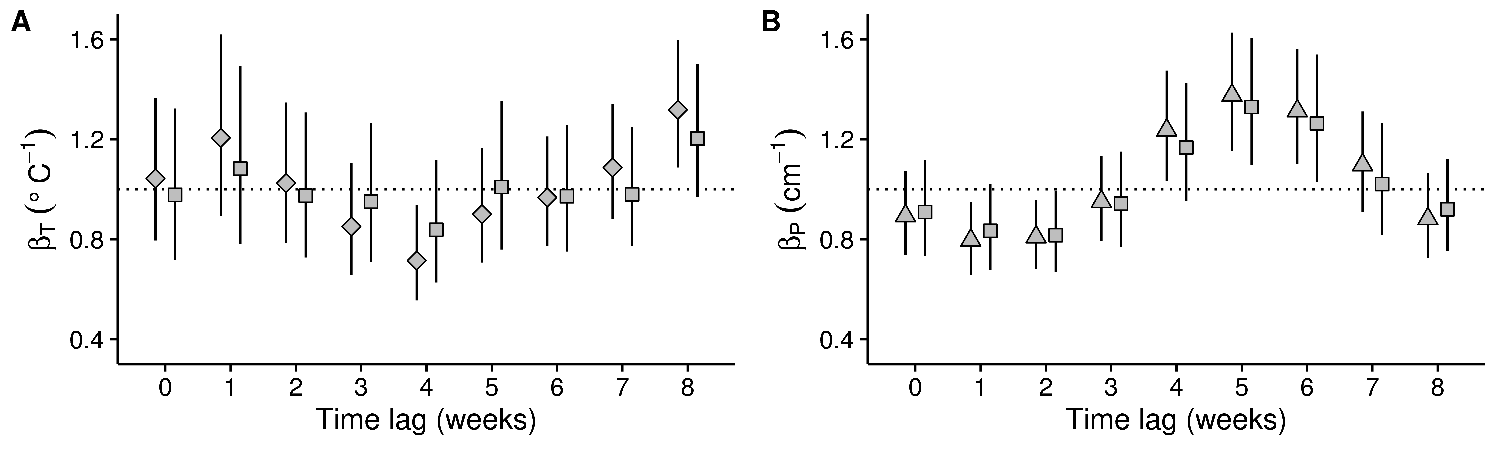
\includegraphics[width=.75\linewidth]{figures/Fig5_revised2.pdf}
\captionof{figure}{{Effect of a variation of 1$^{\circ}$C of the weekly-averaged mean temperature (panel A) and of 1 cm of the weekly-averaged precipitation (panel B) on transmissibility according to a given time lag.}}
\end{center}


}

%----------------------------------------------------------------------------------------


%----------------------------------------------------------------------------------------
%	RESULTS 2
%----------------------------------------------------------------------------------------

\headerbox{Conclusions}{name=conc,span=2,column=1,below=results2,above=bottom}{ % To reduce this block to 1 column width, remove 'span=2'

We jointly analysed epidemics of Zika and Chikungunya in nine island territories to quantify the respective roles of the virus, the territory and the weather conditions in the outbreak dynamics. We showed that Chikungunya and Zika have similar transmissibility when spreading in the same location. Accounting for the level of precipitation improved the modelling of the epidemic profiles, notably for the outbreaks of Zika in Tahiti and of Chikungunya in the Sous-le-vent Islands. The absence of effect of temperature can be related to the low variability of temperature in these areas. Eventually, different probabilities of developing symptoms for the two diseases translated in substantial differences in reporting rates. The present study provides valuable information for the assessment and projection of \textit{Aedes}-borne infections spread. In addition, it introduces an approach that can be adopted in other comparative analyses involving multiple arboviruses and locations. 
}

%----------------------------------------------------------------------------------------






\end{poster}

\end{document}